\let\negmedspace\undefined
\let\negthickspace\undefined
\documentclass[journal,12pt,twocolumn]{IEEEtran}
\usepackage{gensymb}
\usepackage{amssymb}
\usepackage[cmex10]{amsmath}
\usepackage{amsthm}
\usepackage[export]{adjustbox}
\usepackage{bm}
\usepackage{longtable}
\usepackage{enumitem}
\usepackage{mathtools}
 \usepackage{tikz}
\usepackage[breaklinks=true]{hyperref}
\usepackage{listings}
\usepackage{color}                                            %%
\usepackage{array}                                            %%
\usepackage{longtable}                                        %%
\usepackage{calc}                                             %%
\usepackage{multirow}                                         %%
\usepackage{hhline}                                           %%
\usepackage{ifthen}                                           %%
\usepackage{lscape}     
\usepackage{multicol}
% \usepackage{enumerate}
\DeclareMathOperator*{\Res}{Res}
\renewcommand\thesection{\arabic{section}}
\renewcommand\thesubsection{\thesection.\arabic{subsection}}
\renewcommand\thesubsubsection{\thesubsection.\arabic{subsubsection}}
\renewcommand\thesectiondis{\arabic{section}}
\renewcommand\thesubsectiondis{\thesectiondis.\arabic{subsection}}
\renewcommand\thesubsubsectiondis{\thesubsectiondis.\arabic{subsubsection}}
\hyphenation{op-tical net-works semi-conduc-tor}
\def\inputGnumericTable{}                                 %%
\lstset{
frame=single, 
breaklines=true,
columns=fullflexible
}
\begin{document}
\newtheorem{theorem}{Theorem}[section]
\newtheorem{problem}{Problem}
\newtheorem{proposition}{Proposition}[section]
\newtheorem{lemma}{Lemma}[section]
\newtheorem{corollary}[theorem]{Corollary}
\newtheorem{example}{Example}[section]
\newtheorem{definition}[problem]{Definition}
\newcommand{\BEQA}{\begin{eqnarray}}
\newcommand{\EEQA}{\end{eqnarray}}
\newcommand{\define}{\stackrel{\triangle}{=}}
\newcommand*\circled[1]{\tikz[baseline=(char.base)]{
    \node[shape=circle,draw,inner sep=2pt] (char) {#1};}}
\bibliographystyle{IEEEtran}
\providecommand{\mbf}{\mathbf}
\providecommand{\pr}[1]{\ensuremath{\Pr\left(#1\right)}}
\providecommand{\qfunc}[1]{\ensuremath{Q\left(#1\right)}}
\providecommand{\sbrak}[1]{\ensuremath{{}\left[#1\right]}}
\providecommand{\lsbrak}[1]{\ensuremath{{}\left[#1\right.}}
\providecommand{\rsbrak}[1]{\ensuremath{{}\left.#1\right]}}
\providecommand{\brak}[1]{\ensuremath{\left(#1\right)}}
\providecommand{\lbrak}[1]{\ensuremath{\left(#1\right.}}
\providecommand{\rbrak}[1]{\ensuremath{\left.#1\right)}}
\providecommand{\cbrak}[1]{\ensuremath{\left\{#1\right\}}}
\providecommand{\lcbrak}[1]{\ensuremath{\left\{#1\right.}}
\providecommand{\rcbrak}[1]{\ensuremath{\left.#1\right\}}}
\theoremstyle{remark}
\newtheorem{rem}{Remark}
\newcommand{\sgn}{\mathop{\mathrm{sgn}}}
\providecommand{\abs}[1]{\left\vert#1\right\vert}
\providecommand{\res}[1]{\Res\displaylimits_{#1}} 
\providecommand{\norm}[1]{\left\lVert#1\right\rVert}
%\providecommand{\norm}[1]{\lVert#1\rVert}
\providecommand{\mtx}[1]{\mathbf{#1}}
\providecommand{\mean}[1]{E\left[ #1 \right]}
\providecommand{\fourier}{\overset{\mathcal{F}}{ \rightleftharpoons}}
%\providecommand{\hilbert}{\overset{\mathcal{H}}{ \rightleftharpoons}}
\providecommand{\system}{\overset{\mathcal{H}}{ \longleftrightarrow}}
	%\newcommand{\solution}[2]{\textbf{Solution:}{#1}}
\newcommand{\solution}{\noindent \textbf{Solution: }}
\newcommand{\cosec}{\,\text{cosec}\,}
\providecommand{\dec}[2]{\ensuremath{\overset{#1}{\underset{#2}{\gtrless}}}}
\newcommand{\myvec}[1]{\ensuremath{\begin{pmatrix}#1\end{pmatrix}}}
\newcommand{\mydet}[1]{\ensuremath{\begin{vmatrix}#1\end{vmatrix}}}
\newcommand*{\permcomb}[4][0mu]{{{}^{#3}\mkern#1#2_{#4}}}
\newcommand*{\perm}[1][-3mu]{\permcomb[#1]{P}}
\newcommand*{\comb}[1][-1mu]{\permcomb[#1]{C}}
\numberwithin{equation}{subsection}
\makeatletter
\@addtoreset{figure}{problem}
\makeatother
\let\StandardTheFigure\thefigure
\let\vec\mathbf
\renewcommand{\thefigure}{\theproblem}
\def\putbox#1#2#3{\makebox[0in][l]{\makebox[#1][l]{}\raisebox{\baselineskip}[0in][0in]{\raisebox{#2}[0in][0in]{#3}}}}
     \def\rightbox#1{\makebox[0in][r]{#1}}
     \def\centbox#1{\makebox[0in]{#1}}
     \def\topbox#1{\raisebox{-\baselineskip}[0in][0in]{#1}}
     \def\midbox#1{\raisebox{-0.5\baselineskip}[0in][0in]{#1}}
\vspace{3cm}
\title{ASSIGNMENT 2}
\author{CS21BTECH11020}
% make the title area
\maketitle
\newpage

\bigskip
\renewcommand{\thefigure}{\theenumi}
\renewcommand{\thetable}{\theenumi}
\renewcommand{\theequation}{\theenumi}
\section{Problem $1(v)$ $ (2018)$}
\begin{enumerate}[label=\thesection.\arabic*.,ref=\thesection.\theenumi]
    \numberwithin{equation}{enumi}
    \numberwithin{equation}{enumi}
    \numberwithin{figure}{enumi}
    \numberwithin{table}{enumi}
    \item Find the value of constant $'k'$ so that the function $f(x)$ defined as:
        \begin{equation*}
            f(x)=\begin{cases}
                \frac{x^2-2x-3}{x+1}, & x\neq -1 \\
                k, & x=-1
            \end{cases}
        \end{equation*}
        is continuous at x=-1.\\
        \solution We have,\\
        \begin{equation}
            f(x)=\begin{cases}
                \frac{x^2-2x-3}{x+1}, & x\neq -1 \\
                k, & x=-1
            \end{cases} \label{eq: 1.1.1}
        \end{equation}
        From Definition of Continuity,\\
        A function $f(x)$ is said to be continuous at $x=a$ iff \\
        \begin{equation}
            f(a^+)=f(a^-)=f(a) \label{eq: 1.1.2}
        \end{equation}
        where,\\
        $f(a^+)=\lim_{h\to 0^+} f(a+h)$\\
        $f(a^-)=\lim_{h\to 0^+} f(a-h)$\\
        Now, In order to make $f(x)$ continuous at \\$x=-1$, It should satisfy equation \eqref{eq: 1.1.2}\\
        we have,
        \begin{equation}
            f(-1^+)=f(-1^-)=f(-1) \label{eq: 1.1.3}
        \end{equation}
        where,
        
            \begin{align}
            f(-1^+) &=\lim_{h\to 0^+}f(-1+h)\\ 
                    &=\lim_{h\to 0^+}\frac{(-1+h)^2-2(-1+h)-3}{(-1+h)+1}\\
                    &=\lim_{h\to 0^+}\frac{h^2-4h}{h} \\
                    &= \lim_{h\to 0^+}h-4 =-4 \label{eq: 1.1.7}
            \end{align}
            \begin{align}
            f(-1^-) &=\lim_{h\to 0^+}f(-1-h)\\ 
                    &=\lim_{h\to 0^+}\frac{(-1-h)^2-2(-1-h)-3}{(-1-h)+1}\\
                    &=\lim_{h\to 0^+}\frac{h^2+4h}{-h} \\
                    &= \lim_{h\to 0^+}-h-4 =-4 \label{eq: 1.1.11}
            \end{align}
            From equation \eqref{eq: 1.1.1}, we have\\
            \begin{equation}
                f(-1)=k \label{eq: 1.1.12}
            \end{equation}
            Putting value from equation \eqref{eq: 1.1.7}, \eqref{eq: 1.1.11} and \eqref{eq: 1.1.12} into \eqref{eq: 1.1.2}, we get\\
            \begin{align}
                f(-1)=k=-4
            \end{align}
            \begin{figure}[!ht]
                \centering
                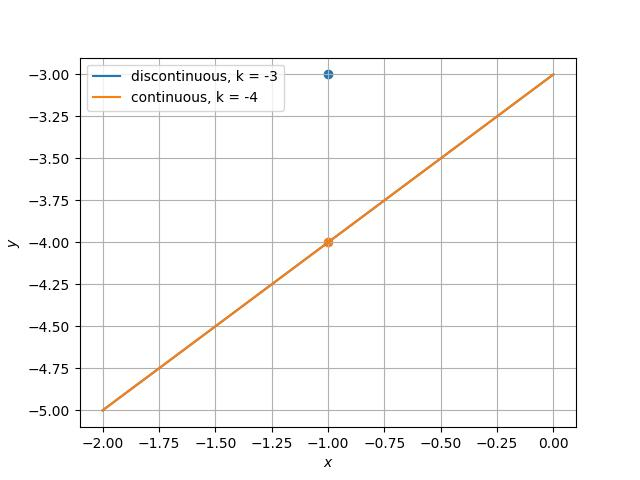
\includegraphics[width=\columnwidth]{continuous.jpg}
                \caption{Function $f(x)$ is discontinuous when $k\neq-4$ but continuous when $k=-4$}
                \label{fig: 1.1.1}
            \end{figure}


\end{enumerate}

\end{document}